\documentclass{ximera}

\usepackage{../OERLinearAlgebra}


\usepackage{mathtools}
\usepackage{tikz-3dplot}
\usetikzlibrary{shapes.geometric}
\usetikzlibrary{arrows}

\author{Anna Davis \and Paul Zachlin} \title{Introduction to Bases} \license{CC-BY 4.0}



\begin{document}
\begin{abstract}
We define bases and consider examples of bases of $\RR^n$ and subspaces of $\RR^n$.
\end{abstract}
\maketitle

\section*{Coordinate Vectors}
When we first introduced vectors we learned to represent them using component notation.  If $\vec{u}=\begin{bmatrix}2\\5\end{bmatrix}$ we know that the head of $\vec{u}$ is located at the point $(2, 5)$.  But there is another way to look at the component form.  Observe that $\vec{u}$ can be expressed as a linear combination of the standard unit vectors $\vec{i}$ and $\vec{j}$:
$$\vec{u}=2\begin{bmatrix}1\\0\end{bmatrix}+5\begin{bmatrix}0\\1\end{bmatrix}=2\vec{i}+5\vec{j}$$
In fact, any vector $\vec{v}=\begin{bmatrix}a\\b\end{bmatrix}$ of $\RR^2$ can be written as a linear combination of $\vec{i}$ and $\vec{j}$:
$$\vec{v}=\begin{bmatrix}a\\b\end{bmatrix}=a\vec{i}+b\vec{j}$$
This gives us an alternative way of interpreting the component notation:
$$\left[\begin{array}{c}  
 a\\b
 \end{array}\right]
 \begin{array}{c}
 
 \longleftarrow\\
 \longleftarrow

 \end{array}
\begin{array}{c}  
 \mbox{coefficient in front of $\vec{i}$}\\\mbox{coefficient in front of $\vec{j}$}
 \end{array}$$
 
 We say that $a$ and $b$ are \dfn{coordinates} of $\vec{v}$ with respect to $\{\vec{i}, \vec{j}\}$, and $\begin{bmatrix}a\\b\end{bmatrix}$ is said to be the \dfn{coordinate vector} for $\vec{v}$ with respect to $\{\vec{i}, \vec{j}\}$.  Every vector $\vec{v}$ of $\RR^2$ can be thus represented using $\vec{i}$ and $\vec{j}$.  Moreover, such representation in terms of $\vec{i}$ and $\vec{j}$ is unique for each vector, meaning that we will never have two different coordinate vectors representing the same vector. We will refer to $\{\vec{i}, \vec{j}\}$ as a \dfn{basis} of $\RR^2$.  
 
 The order in which the basis elements are written matters.  For example, $\vec{u}$ is represented by the coordinate vector $\begin{bmatrix}2\\5\end{bmatrix}$ with respect to $\{\vec{i}, \vec{j}\}$, but changing the basis to $\{\vec{j}, \vec{i}\}$ would change the coordinate vector to $\begin{bmatrix}5\\2\end{bmatrix}$.
 
 $$\left[\begin{array}{c}  
 5\\2
 \end{array}\right]
 \begin{array}{c}
 
 \longleftarrow\\
 \longleftarrow

 \end{array}
\begin{array}{c}  
 \mbox{coefficient in front of the first basis element }\\\mbox{coefficient in front of the second basis element}
 \end{array}$$
 
 Clearly, standard unit vectors $\vec{i}$ and $\vec{j}$ are very convenient, but other vectors can also be used in place of $\vec{i}$ and $\vec{j}$ to represent $\vec{u}$.
 
 \begin{initprob}
 The diagram below shows $\vec{u}$ together with vectors $\vec{w}_1$ and $\vec{w}_2$.
 
 
 \begin{image}[3in]
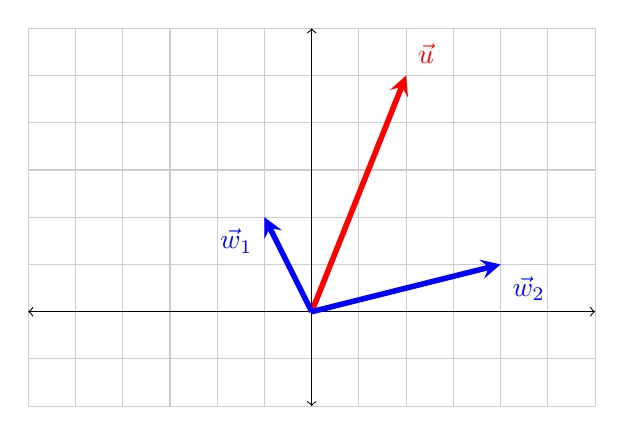
\begin{tikzpicture}[scale=0.6]
\draw[thin,gray!40] (-6,-2) grid (6,6);
  \draw[<->] (-6,0)--(6,0);
  \draw[<->] (0,-2)--(0,6);
  
  \draw[line width=2pt,red,-stealth](0,0)--(2,5) node[above right]{$\vec{u}$};
  \draw[line width=2pt,blue,-stealth](0,0)--(-1,2) node[below left]{$\vec{w}_1$};
  \draw[line width=2pt,blue,-stealth](0,0)--(4,1) node[below right]{$\vec{w}_2$};

 \end{tikzpicture}
\end{image}
 

Using Procedure \ref{pro:lincombgeo} of VEC-M-0040, we can determine that 
$$\vec{u}=2\vec{w}_1+\vec{w}_2$$
as shown below.
\begin{image}[3in]
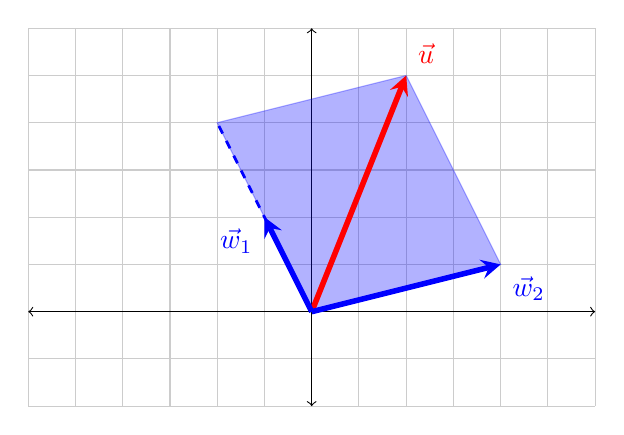
\begin{tikzpicture}[scale=0.6]
\draw[thin,gray!40] (-6,-2) grid (6,6);
  \draw[<->] (-6,0)--(6,0);
  \draw[<->] (0,-2)--(0,6);
  
  \filldraw[blue, opacity=0.3](0,0)--(4,1)--(2,5)--(-2,4)--cycle;
  
  \draw[line width=2pt,red,-stealth](0,0)--(2,5) node[above right]{$\vec{u}$};
  \draw[line width=2pt,blue,-stealth](0,0)--(-1,2) node[below left]{$\vec{w}_1$};
  \draw[line width=2pt,blue,-stealth](0,0)--(4,1) node[below right]{$\vec{w}_2$};
  
   \draw[line width=1pt,blue,dashed](0,0)--(-2,4);

 \end{tikzpicture}
\end{image}

If, for the sake of argument, we declare $\{\vec{w}_1, \vec{w}_2\}$ to be a basis of $\RR^2$, then we can say that the coordinate vector for $\vec{u}$ with respect to $\{\vec{w}_1, \vec{w}_2\}$ is 
$\begin{bmatrix}2\\1\end{bmatrix}$ .

$$\left[\begin{array}{c}  
 2\\1
 \end{array}\right]
 \begin{array}{c}
 
 \longleftarrow\\
 \longleftarrow

 \end{array}
\begin{array}{c}  
 \mbox{coefficient in front of the first basis element }\\\mbox{coefficient in front of the second basis element}
 \end{array}$$
\end{initprob}

\section*{What Constitutes a Basis?}

In the previous section we had used the term \dfn{basis} without defining it.  Now is the time to pause and think about what we {\it want} a basis to do.  Let's focus on $\RR^n$ and subspaces of $\RR^n$.  What we establish here will easily generalize to other vector spaces.  

% I changed "an arbitrary" to "any" to emphasize the need for a basis to span a vector space

Based on our previous discussion, given any vector $\vec{v}$ of $\RR^n$ (or a subspace $V$ of $\RR^n$), we want to be able to write a coordinate vector for $\vec{v}$ with respect to the given basis of $\RR^n$ (or $V$).  Based on this condition, we will require that basis vectors span $\RR^n$ (or $V$).

For example, consider $\vec{w}_1$ and $\vec{w}_2$ shown below.  

\begin{image}
\tdplotsetmaincoords{70}{130}
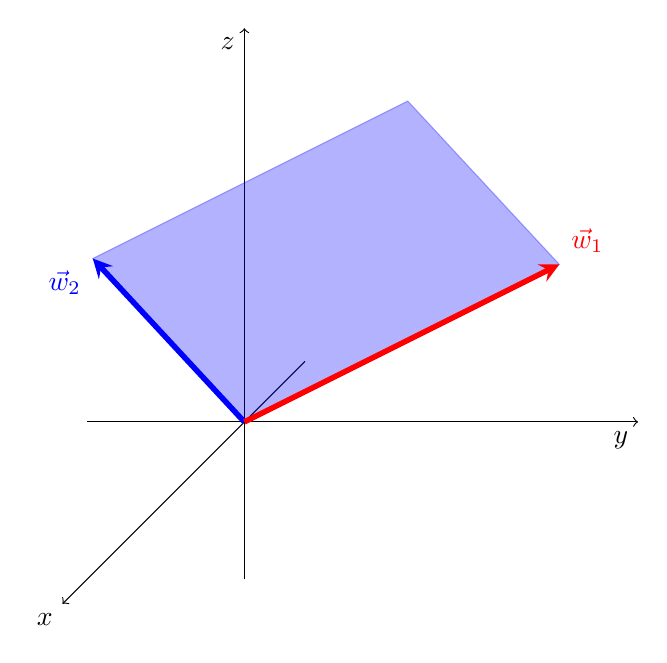
\begin{tikzpicture}
	\draw[->](-2,0,0)--(5,0,0) node[below left]{$y$};
    \draw[->](0,-2,0)--(0,5,0) node[below left]{$z$};
    \draw[->](0,0,-2)--(0,0,6) node[below left]{$x$};
    \filldraw[blue, opacity=0.3] (0,0,0)--(4, 2, 0)--(4,6,5)--(0, 4, 5)--cycle;
    \draw[->, line width=2pt,blue, -stealth](0,0,0)--(0,4,5)node[below left]{$\vec{w}_2$};
    %\draw[line width=1pt,blue, dashed](0,4,0)--(0,4,5);
    %\draw[line width=1pt,blue, dashed](0,0,5)--(0,4,5);
    
    \draw[->, line width=2pt,red, -stealth](0,0,0)--(4,2,0)node[above right]{$\vec{w}_1$};
    
    %\draw[line width=1pt,red, dashed](0,2,0)--(4,2,0);
    %\draw[line width=1pt,red, dashed](4,0,0)--(4,2,0);
    %\draw[->, line width=2pt, -stealth](0,0,0)--(4,6,5)node[above left]{$\begin{bmatrix}5\\4\\6\end{bmatrix}$};
    \end{tikzpicture}
\end{image}
The set $\{\vec{w}_1, \vec{w}_2\}$ cannot be a basis for $\RR^3$ because $\vec{w}_1$ and $\vec{w}_2$ span a plane in $\RR^3$, and any vector not in that plane cannot be written as a linear combination of $\vec{w}_1$ and $\vec{w}_2$.

On the other hand, the plane spanned by $\vec{w}_1$ and $\vec{w}_2$ is a subspace of $\RR^3$.  Because every vector in that plane can be written as a linear combination of $\vec{w}_1$ and $\vec{w}_2$, the set $\{\vec{w}_1, \vec{w}_2\}$ can potentially be a basis for the plane, provided that the set satisfies our second requirement.

Our second requirement is that for a fixed basis of $\RR^n$ (or $V$), the coordinate vector for each $\vec{v}$ in $\RR^n$ (or $V$) should be unique.  Uniqueness of representation in terms of the basis elements will play an important role in our future study of functions that map vector spaces to vector spaces.

The following theorem shows that the uniqueness requirement is equivalent to the requirement that the basis vectors be linearly independent.  %In other words, a basis may not contain redundant vectors.

\begin{theorem}\label{th:linindbasis}
Let $V=\mbox{span}(\vec{w}_1, \vec{w}_2,\ldots,\vec{w}_p)$ be a subspace of $\RR^n$.  Then every element $\vec{v}$ of $V$ has a unique representation as a linear combination of  $\vec{w}_1, \vec{w}_2,\ldots,\vec{w}_p$ if and only if the vectors $\vec{w}_1, \vec{w}_2,\ldots,\vec{w}_p$ are linearly independent.
\end{theorem}
\begin{proof}
Suppose that every $\vec{v}$ in $V$ can be expressed as a unique linear combination of $\vec{w}_1, \vec{w}_2,\ldots,\vec{w}_p$.
This means that $\vec{0}$ has a unique representation as a linear combination of $\vec{w}_1, \vec{w}_2,\ldots,\vec{w}_p$.
But 
$$\vec{0}=0\vec{w}_1+0\vec{w}_2+\ldots+0\vec{w}_p$$
is a representation of $\vec{0}$ in terms of $\vec{w}_1, \vec{w}_2,\ldots,\vec{w}_p$.  Since we are assuming that such a representation is unique, we conclude that there is no other.  This means that the vectors $\vec{w}_1, \vec{w}_2,\ldots,\vec{w}_p$ are linearly independent.

Conversely, suppose that vectors $\vec{w}_1, \vec{w}_2,\ldots,\vec{w}_p$ are linearly independent.  An arbitrary element $\vec{v}$ of $V$ can be expressed as a linear combination of $\vec{w}_1, \vec{w}_2,\ldots,\vec{w}_p$:
$$\vec{v}=a_1\vec{w}_1+a_2\vec{w}_2+\ldots+a_p\vec{w}_p$$
Suppose this representation is not unique.  Then there may be another linear combination that is also equal to $\vec{v}$:
$$\vec{v}=b_1\vec{w}_1+b_2\vec{w}_2+\ldots+b_p\vec{w}_p$$
But then
$$a_1\vec{w}_1+a_2\vec{w}_2+\ldots+a_p\vec{w}_p=b_1\vec{w}_1+b_2\vec{w}_2+\ldots+b_p\vec{w}_p$$
This gives us
$$(a_1-b_1)\vec{w}_1+(a_2-b_2)\vec{w}_2+\ldots+(a_p-b_p)\vec{w}_p=\vec{0}$$
Because we assumed that $\vec{w}_1, \vec{w}_2,\ldots,\vec{w}_p$ are linearly independent, we must have
$$a_1-b_1=0,\, a_2-b_2=0,\,\ldots ,\,a_p-b_p=0$$
so that
$$a_1=b_1,\, a_2=b_2,\,\ldots ,\,a_p=b_p$$
This proves the representation of $\vec{v}$ in terms of $\vec{w}_1, \vec{w}_2,\ldots,\vec{w}_p$ is unique.

\end{proof}


\begin{example}
Let $V=\mbox{span} (\mathcal{S}$) where $\mathcal{S}=\left\{\begin{bmatrix}5\\2\\4\end{bmatrix},\begin{bmatrix}4\\1\\1\end{bmatrix},\begin{bmatrix}-3\\0\\2\end{bmatrix}\right\}$.  Show that $\mathcal{S}$ cannot be a basis of $V$.
% by expressing $\begin{bmatrix}1\\1\\3\end{bmatrix}$ as a linear combination of  $\begin{bmatrix}5\\2\\4\end{bmatrix},\begin{bmatrix}4\\1\\1\end{bmatrix},\begin{bmatrix}-3\\0\\2\end{bmatrix}$ in two different ways.
% \begin{explanation}\label{rref} 
% By observation,
% $$\begin{bmatrix}1\\1\\3\end{bmatrix}=\begin{bmatrix}5\\2\\4\end{bmatrix}+ (-1)\begin{bmatrix}4\\1\\1\end{bmatrix}+0\begin{bmatrix}-3\\0\\2\end{bmatrix} \quad
% and 
% \quad \begin{bmatrix}1\\1\\3\end{bmatrix}=0\begin{bmatrix}5\\2\\4\end{bmatrix}+ \begin{bmatrix}4\\1\\1\end{bmatrix}+\begin{bmatrix}-3\\0\\2\end{bmatrix}$$
% This shows that if we had mistakingly used $\left\{\begin{bmatrix}5\\2\\4\end{bmatrix},\begin{bmatrix}4\\1\\1\end{bmatrix},\begin{bmatrix}-3\\0\\2\end{bmatrix}\right\}$ as a basis for $V$, the vector $\begin{bmatrix}1\\1\\3\end{bmatrix}$ would have at least two coordinate vectors with respect to the proposed basis:
% $$\begin{bmatrix}1\\-1\\0\end{bmatrix}\quad\text{and}\quad\begin{bmatrix}\answer{0}\\\answer{1}\\\answer{1}\end{bmatrix}$$

% In conclusion, we observe that the set $\left\{\begin{bmatrix}5\\2\\4\end{bmatrix},\begin{bmatrix}4\\1\\1\end{bmatrix},\begin{bmatrix}-3\\0\\2\end{bmatrix}\right\}$ is not linearly independent.
% \end{explanation}

\begin{explanation}\label{rref} 
Perhaps you noticed there is more than one way to represent the vector $\begin{bmatrix}1\\1\\3\end{bmatrix}$.  For example, 
\begin{equation}\begin{bmatrix}1\\1\\3\end{bmatrix}=\begin{bmatrix}5\\2\\4\end{bmatrix}+ (-1)\begin{bmatrix}4\\1\\1\end{bmatrix}+0\begin{bmatrix}-3\\0\\2\end{bmatrix} \quad
and 
\quad \begin{bmatrix}1\\1\\3\end{bmatrix}=0\begin{bmatrix}5\\2\\4\end{bmatrix}+ \begin{bmatrix}4\\1\\1\end{bmatrix}+\begin{bmatrix}-3\\0\\2\end{bmatrix}\end{equation}\label{two_ways}
This shows that if we had mistakingly used $\mathcal{S}$ as a basis for $V$, the vector $\begin{bmatrix}1\\1\\3\end{bmatrix}$ would not have a unique coordinate vector with respect to the proposed basis.  Indeed, from the equations in \ref{two_ways}, we may arrive at these coordinate vectors with respect to $\mathcal{S}$:
$$\begin{bmatrix}1\\-1\\0\end{bmatrix}\quad\text{and}\quad\begin{bmatrix}\answer{0}\\\answer{1}\\\answer{1}\end{bmatrix}$$

Since it is difficult to expect that we will ``notice'' that there is more than one way to represent the vector $\begin{bmatrix}1\\1\\3\end{bmatrix}$, the better way to proceed is to make use of Theorem \ref{th:linindbasis}.  We will check to see whether or not the set $\mathcal{S}$ is linearly independent.  To this end, we write the vectors in $\mathcal{S}$ as the columns of a matrix $A$, and apply our row operations until it is in reduced row-echelon form.

$$A=\left[\begin{array}{ccc}  
 5&4&-3\\2&1&0\\4&1&2
 \end{array}\right], \quad \mbox{rref}(A) = \left[\begin{array}{ccc}  
 1&0&1\\0&1&-2\\0&0&0
 \end{array}\right]
$$

When we studied linear independence in Module {\color{red} reference}, we learned that such a calculation shows that the vectors in $\mathcal{S}$ are linearly dependent.  Therefore, by Theorem \ref{th:linindbasis}, there is not a unique representation of $\begin{bmatrix}1\\1\\3\end{bmatrix}$ as a linear combination of the vectors in $\mathcal{S}$.

% From these calculations, we can see that there are in fact infinitely many ways to represent $\begin{bmatrix}1\\1\\3\end{bmatrix}$ as a linear combination of the vectors in $\mathcal{S}$. Observe the following.
% $$B=\left[\begin{array}{ccc|c}  
%  5&4&-3&1\\2&1&0&1\\4&1&2&3
%  \end{array}\right], \quad \mbox{rref}(B) = \left[\begin{array}{ccc|c}  
%  1&0&1&*\\0&1&-2&*\\0&0&0&*
%  \end{array}\right]
% $$
% Our calculations indicate that the system of equations represented by the augmented matrix $B$ has either zero or infinitely many solutions, so we will not have a \underline{unique} way of representing $\begin{bmatrix}1\\1\\3\end{bmatrix}$ as a linear combination of the vectors in $\mathcal{S}$.

% !!! SHORT VIDEO HERE NOW MAY HELP!!!

\end{explanation}
\end{example}


\section*{Definition of a Basis}

\begin{definition}\label{def:basis}
A set $\mathcal{S}$ of vectors is called a \dfn{basis} of $\RR^n$ (or a basis of a subspace $V$ of $\RR^n$) provided that $\mathcal{S}$
\begin{enumerate}
\item \label{item:defbasis1}
Spans $\RR^n$ (or $V$)
\item \label{item:defbasis2}
Is linearly independent
\end{enumerate}
\end{definition}

\begin{example}
The standard unit vectors $\vec{e}_1, \ldots ,\vec{e}_n$ are linearly independent and span $\RR^n$.  Thus $\{\vec{e}_1, \ldots ,\vec{e}_n\}$ is a basis of $\RR^n$.
\end{example}

\begin{definition} The set $\{\vec{e}_1, \ldots ,\vec{e}_n\}$ is called the \dfn{standard basis} of $\RR^n$.
\end{definition}

% \begin{example}
% Let $V=\mbox{span}\left(\begin{bmatrix}-2\\1\\3\end{bmatrix},\begin{bmatrix}2\\-4\\1\end{bmatrix}\right)$.  Prove that $\mathcal{B}=\left\{\begin{bmatrix}-2\\1\\3\end{bmatrix},\begin{bmatrix}2\\-4\\1\end{bmatrix}\right\}$ is a basis for $V$ and find the coordinate vector for $\vec{v}=\begin{bmatrix}2\\-10\\9\end{bmatrix}$ with respect to $\mathcal{B}$.
% \begin{explanation}
% Clearly the two vectors in $\mathcal{B}$ span $V$.  To show that the two vectors are linearly independent, we solve the vector equation:
% $$a_1\begin{bmatrix}-2\\1\\3\end{bmatrix}+a_2\begin{bmatrix}2\\-4\\1\end{bmatrix}=\vec{0}$$
% The augmented matrix corresponding to this equation reduces as follows:
% $$\left[\begin{array}{cc|c}  
%  -2&2&0\\-1&-4&0\\3&1&0
%  \end{array}\right]\rightsquigarrow\left[\begin{array}{cc|c}  
%  1&0&0\\0&1&0\\0&0&0
%  \end{array}\right]$$
%  This gives us $a_1=a_2=0$, and we conclude that the two elements of $\mathcal{B}$ are linearly independent.  By Definition \ref{def:basis}, $\mathcal{B}$ is a basis of $V$.
 
%  To find the coordinate vector for $\begin{bmatrix}2\\-10\\9\end{bmatrix}$ with respect to $\mathcal{B}$, we need to express $\begin{bmatrix}2\\-10\\9\end{bmatrix}$ as a linear combination of the elements of $\mathcal{B}$.  To this end, we need to solve the vector equation:
%  $$a_1\begin{bmatrix}-2\\1\\3\end{bmatrix}+a_2\begin{bmatrix}2\\-4\\1\end{bmatrix}=\begin{bmatrix}2\\-10\\9\end{bmatrix}$$
%  The augmented matrix and the reduced row-echelon form are:
%  $$\left[\begin{array}{cc|c}  
%  -2&2&2\\-1&-4&-10\\3&1&9
%  \end{array}\right]\rightsquigarrow\left[\begin{array}{cc|c}  
%  1&0&2\\0&1&3\\0&0&0
%  \end{array}\right]$$
%  We conclude that $a_1=2$, $a_2=3$.  This gives us
%  $$2\begin{bmatrix}-2\\1\\3\end{bmatrix}+3\begin{bmatrix}2\\-4\\1\end{bmatrix}=\begin{bmatrix}2\\-10\\9\end{bmatrix}$$
%  The coefficient in front of the first basis vector is $2$, the coefficient in front of the second basis vector is $3$.  This means that the coordinate vector for $\begin{bmatrix}2\\-10\\9\end{bmatrix}$ with respect to $\mathcal{B}$ is $\begin{bmatrix}2\\3\end{bmatrix}$.
 
%  It may seem strange to you that the coordinate vector for a vector in $\RR^3$ only has two components.  But remember that subspace $V$ is a plane.  When viewed as a vector in the plane, it  makes sense that the coordinate vector for $\begin{bmatrix}2\\-10\\9\end{bmatrix}$ only requires two components.  This issue is related to the question of dimension, which will be addressed in a subsequent module.
% \end{explanation}
% \end{example}

\begin{example}
Let $V=\mbox{span}\left(\begin{bmatrix}-2\\1\\3\end{bmatrix},\begin{bmatrix}2\\-4\\1\end{bmatrix}\right)$.  It is easy to see that $$\mathcal{B}=\left\{\begin{bmatrix}-2\\1\\3\end{bmatrix},\begin{bmatrix}2\\-4\\1\end{bmatrix}\right\}$$ is a basis for $V$ because the two vectors in $\mathcal{B}$ are linearly independent and span $V$.  Find the coordinate vector for $\vec{v}=\begin{bmatrix}2\\-10\\9\end{bmatrix}$ with respect to $\mathcal{B}$.
\begin{explanation}
We need to express $\begin{bmatrix}2\\-10\\9\end{bmatrix}$ as a linear combination of the elements of $\mathcal{B}$.  To this end, we need to solve the vector equation:
 $$a_1\begin{bmatrix}-2\\1\\3\end{bmatrix}+a_2\begin{bmatrix}2\\-4\\1\end{bmatrix}=\begin{bmatrix}2\\-10\\9\end{bmatrix}$$
 The augmented matrix and the reduced row-echelon form are:
 $$\left[\begin{array}{cc|c}  
 -2&2&2\\-1&-4&-10\\3&1&9
 \end{array}\right]\rightsquigarrow\left[\begin{array}{cc|c}  
 1&0&2\\0&1&3\\0&0&0
 \end{array}\right]$$
 We conclude that $a_1=2$, $a_2=3$.  This gives us
 $$2\begin{bmatrix}-2\\1\\3\end{bmatrix}+3\begin{bmatrix}2\\-4\\1\end{bmatrix}=\begin{bmatrix}2\\-10\\9\end{bmatrix}$$
 The coefficient in front of the first basis vector is $2$, the coefficient in front of the second basis vector is $3$.  This means that the coordinate vector for $\begin{bmatrix}2\\-10\\9\end{bmatrix}$ with respect to $\mathcal{B}$ is $\begin{bmatrix}2\\3\end{bmatrix}$.
 
 It may seem strange to you that the coordinate vector for a vector in $\RR^3$ only has two components.  But remember that subspace $V$ is a plane.  When viewed as a vector in the plane $V$, it  makes sense that the coordinate vector for $\begin{bmatrix}2\\-10\\9\end{bmatrix}$ only requires two components.  This issue is related to the question of dimension, which will be addressed in a subsequent module.
\end{explanation}
\end{example}


\section*{Practice Problems}
\begin{problem}
Let $\mathcal{B}=\left\{\begin{bmatrix}1\\1\end{bmatrix},\begin{bmatrix}-1\\2\end{bmatrix}\right\}$ be a basis for $\RR^2$.  (Do a mental verification that $\mathcal{B}$ is a basis.)  For each $\vec{v}$ given below, find the coordinate vector for $\vec{v}$ with respect to $\mathcal{B}$.
  \begin{problem}
 Vector $\vec{v}$. 
  \begin{image}[2in]
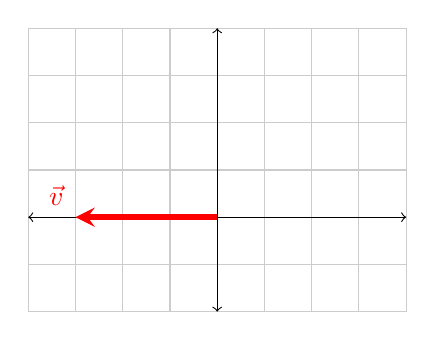
\begin{tikzpicture}[scale=0.6]
\draw[thin,gray!40] (-4,-2) grid (4,4);
  \draw[<->] (-4,0)--(4,0);
  \draw[<->] (0,-2)--(0,4);
   \draw[line width=2pt,red,-stealth](0,0)--(-3,0) node[above left]{$\vec{v}$};
   \end{tikzpicture}
\end{image}

Answer:
$$\begin{bmatrix}\answer{-2}\\\answer{1}\end{bmatrix}$$
  \end{problem}
  
  \begin{problem}
  Vector $\vec{v}$.
  \begin{image}[1.5in]
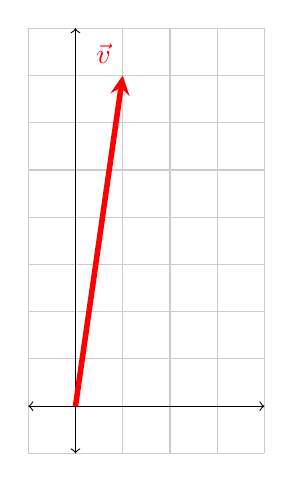
\begin{tikzpicture}[scale=0.6]
\draw[thin,gray!40] (-1,-1) grid (4,8);
  \draw[<->] (-1,0)--(4,0);
  \draw[<->] (0,-1)--(0,8);
   \draw[line width=2pt,red,-stealth](0,0)--(1,7) node[above left]{$\vec{v}$};
   \end{tikzpicture}
\end{image}
Answer:
$$\begin{bmatrix}\answer{3}\\\answer{2}\end{bmatrix}$$
  \end{problem}
\end{problem}

\begin{problem}
Let $\mathcal{B}=\left\{\begin{bmatrix}1\\-1\\3\end{bmatrix},\begin{bmatrix}2\\1\\-1\end{bmatrix}\right\}$ be a basis for 
$\mbox{span}\left(\begin{bmatrix}1\\-1\\3\end{bmatrix},\begin{bmatrix}2\\1\\-1\end{bmatrix}\right)$.  Find the coordinate vector for $\begin{bmatrix}-4\\-2\\2\end{bmatrix}$ with respect to $\mathcal{B}$.

Answer:
$$\begin{bmatrix}\answer{0}\\\answer{-2}\end{bmatrix}$$
\end{problem}

\begin{problem}
Suppose $\mathcal{B}=\left\{\begin{bmatrix}1\\1\\1\end{bmatrix},\begin{bmatrix}1\\0\\1\end{bmatrix}, \vec{w}\right\}$ is a basis for $\RR^3$.  Find $\vec{w}$ if the coordinate vector for $\begin{bmatrix}-2\\-7\\4\end{bmatrix}$ is $\begin{bmatrix}-1\\2\\-3\end{bmatrix}$.

Answer:
$$\begin{bmatrix}\answer{1}\\\answer{2}\\\answer{-1}\end{bmatrix}$$
\end{problem}

\begin{problem}

Which of the following is a basis for $\RR^2$? 

\begin{selectAll}
  \choice{$\left\{\begin{bmatrix}1\\1\end{bmatrix},\begin{bmatrix}-1\\-1\end{bmatrix}, \begin{bmatrix}1\\2\end{bmatrix}\right\}$}
  \choice[correct]{$\left\{\begin{bmatrix}1\\1\end{bmatrix}, \begin{bmatrix}1\\2\end{bmatrix}\right\}$}
  \choice{$\left\{\begin{bmatrix}3\\-1\end{bmatrix},\begin{bmatrix}1\\2\end{bmatrix}, \begin{bmatrix}-4\\3\end{bmatrix}\right\}$}
   \choice{$\left\{\begin{bmatrix}1\\-3\end{bmatrix}, \begin{bmatrix}-2\\6\end{bmatrix}\right\}$}
  \end{selectAll}
\end{problem}

\begin{problem}

Which of the following is a basis for $V=\mbox{span}\left(\begin{bmatrix}1\\1\\1\end{bmatrix}, \begin{bmatrix}1\\-2\\1\end{bmatrix}\right)$? 

\begin{selectAll}
  \choice[correct]{$\left\{\begin{bmatrix}2\\-1\\2\end{bmatrix},\begin{bmatrix}1\\-2\\1\end{bmatrix}\right\}$}
  \choice[correct]{$\left\{\begin{bmatrix}0\\3\\0\end{bmatrix}, \begin{bmatrix}3\\-3\\3\end{bmatrix}\right\}$}
  \choice{$\left\{\begin{bmatrix}1\\0\\0\end{bmatrix},\begin{bmatrix}0\\0\\1\end{bmatrix}\right\}$}
  \choice{$\left\{\begin{bmatrix}1\\1\\1\end{bmatrix},\begin{bmatrix}2\\-1\\2\end{bmatrix}, \begin{bmatrix}1\\-2\\1\end{bmatrix}\right\}$}
  \end{selectAll}
\end{problem}
\end{document}
